\documentclass{article}

\usepackage{fullpage}
\usepackage{amsmath,amssymb}
\usepackage{graphicx,subfigure}
%\usepackage[utf8]{inputenc}


\def\x{\mathbf{x}}
\def\y{\mathbf{y}}
\def\e{\mathbf{e}}
\def\th{{\boldsymbol{\theta}}}
\def\n{{\boldsymbol{\nu}}}
\def\u{\mathbf{u}}
\def\m{\mathbf{m}}
\def\v{\mathbf{v}}
\def\f{\mathbf{f}}
\def\E{\mathbb{E}}
\def\g{\mathbf{g}}
\def\h{\mathbf{h}}
\def\A{\mathbf{A}}
\def\B{\mathbf{B}}
\def\prec{\mathrm{prec}}

\title{Variational sampling reloaded}
\author{Alexis Roche}
%\date{}

\usepackage{natbib}
\usepackage{graphicx}

\begin{document}

\maketitle


\section{Introduction}

Variational sampling is a simple and general method for computational statistics that extends in a rather natural way the basic importance sampling method, aka Monte Carlo integration, which dates back (at least) to World War II.

I discovered it in 2010 while trying to interpret importance sampling in a variational framework, and coined the name ``variational sampling'' as a result of that. Despite its relative simplicity, it did not seem to be known under any name in the literature, which puzzled me back then, and keeps puzzling me. 

There could only be two reasons for that. Either it was a bad idea, or researchers had overlooked it. I was crazy enough to believe in the latter explanation.

Hence, I tried hard to publish it in NIPS, but failed four times in as many attempts from 2010 to 2016. I did publish it on arXiv in May 2011 on the advice of Pr Nanny Wermuth, who had come across my work and encouraged me to push it forward, and later in a low cost e-journal nicely called {\em International Journal of Advanced Statistics and Probability} in a desperate, yet successful, attempt to make at least one peer-reviewed publication on the topic.

As of May 2024, these papers have a total of 4 citations in Google Scholar, including 2 self-citations. 

Variational sampling is, unquestionably, the worst failure of my whole researcher career in terms of scientific impact, that being said while said career operates on reasonably modest standards.

%%%, but much simpler than many advanced sampling and approximate inference methods found in the literature.
%thought it should be part of any standard computational statistics toolbox


\section{History}

How the pieces of the puzzle came together.
\begin{itemize}
\item 2010: discovery of the VS core idea and its intriguing exactness property.
\item 2011--13: consolidation of the theory behind VS.
\item 2014--16: realization that VS is useful in practice combined with Expectation Propagation.
\item 2018--19: extension to large dimension via custom optimizer (avoiding big Hessian inversion); unveiling connection between distribution scaling and $\alpha$-divergence minimization.
\item 2022: proven bound on VS asymptotic variance.
\item 2023: revisited custom optimizer.
\end{itemize}


\section{Variational sampling recap}

Consider:
\begin{itemize}
\item a reference distribution~$\pi(x)$ (from which we can sample)
\item a factor~$f(x)$ so that $p\equiv \pi f$ is a distribution of interest
\item an approximating factor~$g$ searched under the exponential form:
  $$
  g(x) = e^{\theta^\top \phi(x)},
  $$ where $\phi$ is a known vector-valued function and $\theta$ needs
  to be determined.
\end{itemize}

VS is a stochastic method to approximate the parametric factor~$g$ that minimizes the generalized Kullback-Leibler divergence:
$$
D(\pi f\|\pi g)
= \int \pi (f \log \frac{f}{g} + g - f)
$$

It does so by sampling independent points $(x_1,\ldots,x_n)$ from~$\pi$ and minimizing a Monte Carlo approximation to the KL~divergence, leading to the surrogate criterion:
$$
\tilde{D}(\theta) = \frac{1}{n} \sum_i \ell[ f(x_i), g_\theta(x_i) ],
$$
where $\ell(f, g)$ is the loss function associated with the KL~divergence:
$$
\ell(f, g) \equiv f \log \frac{f}{g} - f + g
$$
  
We have proved in our initial paper from 2013 that the resulting estimator of the integral, or moment, $I(\phi) \equiv \int \pi f \phi$, is asymptotically unbiased with variance matrix:
$$
\Sigma_n = \frac{1}{n} \int \pi (f - g_\star)^2 \phi \phi^\top,
$$
where $g_\star$ is the genuine (intractable) KL~minimizer:
$$
g_\star \equiv \arg\min_g D(\pi f\|\pi g).
$$

This makes VS fundamentally different from importance sampling, for which the moment is directly estimated via:
$$
\hat{\mu} \equiv \frac{1}{n} \sum_i f(x_i)\phi(x_i),
$$
yielding an unbiased estimator with asymptotic variance:
$$
\Sigma_n^{IS} = \frac{1}{n} \left[
\int \pi f^2 \phi \phi^\top
- I(\phi) I(\phi)^\top
\right]
$$

In particular, VS has the key consistency property unlike IS to be exact when the target factor lies in the approximating family.

Note, however, that IS can also be seen as a variational sampling instance corresponding to another surrogate criterion:
$$
\tilde{D}_{IS}(\theta)
= - \frac{1}{n} \sum_i f(x_i) \log g_\theta(x_i) 
  + \int \pi g_\theta
.
$$

The key difference with $\tilde{D}(\theta)$ is that the sample mean of $g_\theta(x_i)$ is replaced by its asymptotical value. Hence, $\tilde{D}_{IS}$ may be seen as a ``partial Rao-Blackwellization'' of $\tilde{D}$, partial because we can't do it for the term in $\log g_\theta(x_i)$; and, because it's partial, it may not improve the estimator accuracy (our main claim is that it doesn't in many situations of practical interest).



\section{Variance upper bound}

Intuitively, the closer the target factor~$f$ to the approximating family, the smaller the VS~asymptotic variance. To show that formally, we would like to upper bound the mean square error $\int\pi(f-g)^2$ by some increasing function of the KL~divergence $D(\pi f\|\pi g)$. 

\subsection{VS variance inequality}

I have been bumping into this issue for years... only to realize in January 2022 that such an upper bound does exist and is actually pretty simple to exhibit. We will need a straightforward intermediate result:

\paragraph{Alexis theorem:} if $f:\Omega\in\mathbb{R}\to \mathbb{R}$ is a smooth convex function from some open interval reaching its minimum in $a\in\Omega$, assuming for simplicity that $f(a)=0$, and such that the second derivative $f''$ is a decreasing function, then we have that:
$$
\forall x \leq a,
\qquad
f(x) \geq \frac{1}{2} f''(a) (x - a)^2 .
$$

The proof is straightforward from the fact that $f''(x) \geq f''(a)$ since $f''$ is decreasing, then we just need to integrate this relationship twice and take into account that $f'(a)=f(a)=0$.

Next, let us consider the loss function $\ell(f,g)=f\log(f/g)+g-f$ as a function of $g$. We easily see that:
$$
\frac{\partial\ell}{\partial g} = 1 - \frac{f}{g},
\qquad
\frac{\partial^2\ell}{\partial g^2} = \frac{f}{g^2},
$$
implying that the loss is not only convex in~$g$ but also satisfies the conditions of Alexis's theorem with $a=f$. Hence,
$$
\forall g\leq f,
\qquad
\ell(f, g) \geq \frac{1}{2f} (g - f)^2. 
$$

But we can also consider the loss as a function of~$f$ at fixed~$g$. We have:
$$
\frac{\partial\ell}{\partial f} = \log(f),
\qquad
\frac{\partial^2\ell}{\partial g^2} = \frac{1}{f},
$$
which means that Alexis's theorem can be applied again, this time with $a=g$, yielding:
$$
\forall f\leq g,
\qquad
\ell(f, g) \geq \frac{1}{2g} (f - g)^2. 
$$

Concatenating both results, we see that for all $(f, g)$:
$$
(f-g)^2 \leq 2 \max(f, g)\ell(f, g).
$$

Integrating this over~$\pi$, we get this long-waited inequality:
\begin{equation}
\label{eq:variance_inequality}
\int \pi (f-g)^2 \leq 2\max(\|f\|_\infty, \|g\|_\infty) D(\pi f\|\pi g),
\end{equation}
where the infinite norms are taken on the support of~$\pi$, which is infinite if $\pi$ is a Gaussian kernel.

Note that this is only tight if $\max(f,g)$ is constant. The inequality tells us, as intuition suggests, that the mean squared error between factors smoothly goes to zero as the KL~divergence vanishes. But this holds under the condition that both~$f$ and~$g$ remain bounded on the support of~$\pi$. While this may be problematic if~$\pi$ has infinite support, we can just truncate~$\pi$ to guarantee the finiteness of the upper bound at the price of some possibly small bias. As noted in the 2013 paper, this boils down to using a localized version of the KL divergence as the target metric. It may also be justified in terms of a Bayesian prior, and may be a very reasonable thing to do. However, while removing the concern that the VS variance may be infinite, it doesn't prevent it in practice from being very large and yielding
hopelessly slow convergence.

The above inequality gives a variance upper bound on the zero-order moment (the normalizing constant). More generally, consider a positive real $\phi_i$. The above result implies straighforwardly:
$$
(f-g)\phi_i^2
\leq 2 \max(f\phi_i, g\phi_i) \ell(f\phi_i, g\phi_i)
= 2 \max(f\phi_i, g\phi_i) \phi_i\ell(f, g)
= 2 \max(f\phi_i^2, g\phi_i^2) \ell(f, g)
$$
where we use the fact that $\ell(f\phi_i,g\phi_i)=\phi_i\ell(f,g)$. A more general inequality follows by integration, which I would happily call Alexis' inequality:
$$
\int \pi (f-g)^2\phi_i^2 \leq 2\max(\|f\phi_i^2\|_\infty, \|g\phi_i^2\|_\infty) D(\pi f\|\pi g).
$$

This yields the same kind of variance upper bound for any moment estimator we have.


\subsection{Sufficient conditions for VS convergence}

Substituing~$g$ with the minimizer~$g_\star$ of $D(\pi f\|\pi g)$ in the inequality~(\ref{eq:variance_inequality}), we get an upper bound for the VS 0-order moment estimate asymptotic variance:
$$
\int \pi (f-g_\star)^2
\leq
2\max(\|f\|_\infty, \|g_\star\|_\infty)
D(\pi f\|\pi g_\star)
.
$$

Obviously, a sufficient condition for the left-hand side to be finite is that the right-hand side be finite.

We note that, if $\|f\|_\infty$ is finite, then $D(\pi f\|\pi g_\star)$ is finite. The reason is that, by construction, $g_\star$ minimizes the KL~divergence on a function space that contains the constant function $g\equiv 1$, therefore:
$$
D(\pi f\|\pi g_\star)
\leq
D(\pi f\|\pi 1)
=
\int \pi (f\log f - f + 1)
.
$$

Now, the function $x\log x - x + 1$ is positive-valued on $\mathbb{R}_+$, decreasing from 1 to 0 between 0 and 1, and increasing to infinity from 1. It follows that $(f\log f - f + 1)\leq \max(1, \|f\|_\infty \log \|f\|_\infty - \|f\|_\infty + 1)$, hence the KL~divergence term is finite since it is upper bounded by a finite constant:
$$
D(\pi f\|\pi g_\star) \leq
\max(1, \|f\|_\infty \log \|f\|_\infty - \|f\|_\infty + 1)
.
$$

Is the condition $\|f\|_\infty$ finite sufficient?

For the IS estimate, it is -- because the asymptotic variance is related to the variance of $f(x)$ under $\pi(x)$:
$$
{\rm Var}[f(X)]
= \min_{c\in\mathbb{R}} \int \pi (f - c)^2,
$$
which is easily seen to be finite whenever $f$ is upper bounded. 

For VS, however, we need $\|g_\star\|_\infty$ to be finite too. Intuitively, since $g_\star$ is the best fit to $f$ in the KL~sense, the residuals $f-g_\star$ tend to be much smaller than wrt a constant baseline, so we expect $\int \pi(f-g_\star)^2$ to be quite smaller than ${\rm Var}[f(X)]$. We can make this a little bit more precise using :
$$
\min_g \int \pi (f-g)^2 \leq \min_{c\in\mathbb{R}} \int \pi (f-c)^2 = {\rm Var}[f(X)].
$$

However, $g_\star$ does not minimize $\pi (f-g)^2$, it minimizes the KL divergence $D(\pi f\|\pi g)$, therefore the above reasoning doesn't work.

So let's go back to the KL~minimization. One thing we can note is that the variances of $\pi f$ and $\pi g_\star$ are the same owing to the moment matching property of KL~minimization, and so are the precisions:
$$
\prec(\pi g_\star) = \prec(\pi f).
$$

Now, both $\pi$ and $g_\star$ are log-quadratic functions so the precisions add up:
$$
\prec(\pi g_\star) = \prec(\pi) + \prec(g_\star).
$$

Clearly, $\|g_\star\|_\infty$ is finite iff $\prec(g_\star)$ is positive (not necessarily positive definite). This is the case iff: 
$$
\prec(\pi f) \succeq \prec(\pi)
.
$$

In other words, sufficient conditions for VS to converge are:
\begin{enumerate}
\item The factor $f$ is upper bounded.
\item The ``posterior'' variance is smaller than the ``prior'' variance.
\end{enumerate}

Is the second condition implied by the first? No, it isn't.


\paragraph{Damning counter-example.}

Here is a simple one-dimensional counter-example where $\|f\|_\infty$ is finite and $\|g_\star\|_\infty$ is not. Consider a normalized Gaussian reference $\pi = N(0,1)$, and a uniform factor defined by $f = \chi(-a,a)/\pi$, where $a$ is a positive constant, so that the target distribution $\pi f$ is the uniform distribution $\chi(-a,a)$ and its variance is therefore $a^2/ 3$. Following the same reasoning as above, we see that the precision of the fitted factor is:
$$
\prec(g_\star) = \frac{3}{a^2} - 1,
$$
which, for $a$ sufficiently large, namely $a>\sqrt{3}$, is strictly negative, implying that $g_\star$ is not upper bounded. Even worse than that, $g_\star$ goes very fast to infinity as $x$ departs from $0$, so $\int \pi g_\star^2$ is infinite, implying that $\int \pi (f-g_\star)^2$ is also infinite, implying that VS does not converge! 

In this case, the optimal fit $g_\star$ goes to infinity while $f$ vanishes. This is weird. But it happens because, on the one hand, the factor looks like a U-shaped function in the context defined by $\pi$, and, on the other hands, the loss incurred in regions where the factor vanihes, $\ell(0,g)=g$, is only linear in~$g$, so it's ``mild'' even for large values of~$g$ when weighted by~$\pi$. This is consistent with the fact that the KL~divergence is an inclusive  measure (``zero avoiding'' for $g_\star$). In contrast, minimizing $\pi(f-g)^2$ would yield a well-behaved (bell-shaped) factor approximation -- to see this, just realize that $\inf_g\int\pi(f-g)^2 \leq \int\pi f^2$, which is finite.  


\paragraph{Wrapping up.}

We learn several things from the above counter-example.

First off, VS is not necessarily better than IS (it may not converge at all while IS converges).

Second, the intuition that $g_\star$ follows $f$ closely is not necessarily correct. 

Third, this intuition may not be correct even though the factor is ``almost'' perfectly log-quadratic on the domain defined by $\pi$. In the counter-example, VS will do a good job in practice (much better than IS). Why? Just think about it: because on a finite sample drawn from $\pi$, chances are that we don't get any point outside $[-a,a]$, where $f$ is perfectly log-quadratic. 

%For instance, drawing 100000 points from a normal distribution, we have almost no chance to have any point more than 5 times standard deviations away from the mean. With 1000000 points, the same goes for 6 standard deviations.

Hence, and that's a 4th take-away, the asymptotic variance does not tell us the whole truth about how VS performs in practice. The sample size required to reach asymptotic regime may heavily depend on the factor at hand. Besides, the fact that VS may actually worsen by increasing the sample size is both unexpected and concerning.

As already pointed out, truncating the reference distribution doesn't really solve the problem. The asymptotic variance would become finite, but still possibly way too big. In the counter-example, how would we know beforehand that we should truncate outside $[-a,a]$?

So, how can we work around this problem?

%we can put the blame on both the factor for being far off the approximating family and the context $\pi$ as for being too narrow to ``see'' $f$ globally. But we may not know that beforehand.


%Then comes a natural question: when is the variance of $(f-g_\star)$ smaller than that of $f$ under~$\pi$?




\paragraph{Bullshite.}

From this point, can we give practical sufficient conditions for VS convergence?  Convergence in distribution will occur under mild conditions if the integral $\int \pi (f-g_\star)^2\phi\phi^\top$ is finite. The above inequality relating the VS variance to the KL~divergence tells us that this holds whenever $\pi$ has finite support.

What if~$\pi$ is stricly Gaussian, hence doesn't have finite support? 

Similarly to IS, the condition that $f$ is upper bounded is sufficient for $\pi f^2 \phi\phi^\top$ to be finite, and may be easy to fulfill in practice.

We are left with another sufficient condition (which IS doesn't have): that $\pi g_\star^2 \phi\phi^\top$ be finite too. Due to the log-quadratic nature of both $\pi$ and $g_\star$, this holds iff $\pi g_\star$ is Gaussian (i.e. its hegated log is a positive definite quadratic form).

In 1D, let us denote $s^2$ and $\sigma^2$ the respective variances of $\pi$ and $\pi g_\star$. Clearly, $\sigma^2$ is finite because it is equal to the variance of $\pi f$ by the moment matching constraint, which is finite if $f$ is upper bounded. A simple asymptotic analysis then shows that the condition that $\pi g_\star^2$ has finite integral boils down to:
$$
\prec(\pi) + 2 [\prec(\pi f) - \prec(\pi)] > 0,
\quad \Rightarrow \quad
\prec(\pi) < 2 \prec(\pi f),
$$
where $\prec$ denotes the precision, {\em i.e.}, the inverse variance. The condition boils down to:
$$
s^2 > \frac{\sigma^2}{2}.
$$

The same reasoning can be extended in multiple dimension. If we use factorized Gaussians for fitting, the above condition simply applies to each axis.

In short, the kernel size cannot be too small compared to the target distribution. However, we don't know $\sigma$, so how can we guarantee this in practice? 

Let now consider a damping factor $0\leq \alpha \leq 1$, and raise our factor~$f$ to the power~$\alpha$. 


is practically rules out the naive application of VS to unbounded importance weight functions, hence the need to perform VS within a constrained framework such as Expectation Propagation.



Note that, if~$f$ is such that all the moments $\int\pi f \phi$ exist, the same goes for $g_\star$ in virtue of the moment matching condition, implying under very mild conditions on the approximating family, that $g_\star$ is upper bounded (easy to see in the Gaussian case, which is BTW the only one we have considered in practice so far.


\section{Custom optimizer}

We shall note that the basis functions $\phi_i$ underlying the fitting family are somewhat arbitrary, hence comes a natural question: which basis is most convenient for optimization?

Consider for now the case of the KL divergence $D(\theta)=D(\pi f\|\pi g_\theta)$ for a given set of $\phi$-functions. We have the relations:
$$
\nabla D = \int \pi (g_\theta-f) \phi,
\qquad
\nabla^2 D = \int \pi g_\theta \phi\phi^\top.
$$

From there, a key remark is that the Hessian at a particular $\theta$ is the identity matrix if $\phi$ defines an orthonormal basis for the dot product:
$$
\langle h_1, h_2 \rangle \equiv \int \pi g_{\theta} h_1 h_2,
$$
where $h_1$ and $h_2$ are real-valued functions... We have some Hilbert space structure here, but I'll skip these details for now as I am not a mathematician. What really matters is that the Hessian being the identity means that a Newton iteration is very easy to compute as it boils down to a first-order gradient iteration. Importantly, however, this property is achieved for a particular basis function that is {\em dependent on the current fit estimate}.

So, let's say that we have a current fit $g_n$ (which may be defined, for instance, by its coordinates in the canonical, fixed basis) and we want to perform one Newton iteration to improve it. Given an orthonormal basis $\phi_n$ associated with $g_n$ (in the sense of the above-defined dot product), we may look for the update under the form $g_\nu = g_n \exp({\nu^\top \phi_n})$. The Newton iteration from $\nu=0$ then takes the form:
$$
\hat{\nu} = -\lambda \nabla D(0) = \lambda \int \pi(f - g_n)\phi_n,
$$
for some damping factor $\lambda > 0$ (the genuine Newton iteration corresponds to $\lambda=1$), yielding the update:
$$
g_{n+1} = g_n \exp (\hat{\nu}^\top \phi_n).
$$

We will further need to represent $g_{n+1}$ in the same fixed coordinate system as $g_n$, i.e. using a ``$\theta$ parameter'', which will require a linear coordinate change from $\phi_n$ to the fixed basis. 



\subsection{Orthonormal basis}

Let's start in one dimension for simplicity. Given a current fit $g$, let $q=\pi g$ (pig\'e?),  with integral, mean and scale parameters $(Z, m, s)$, the following three functions define an orthonormal basis:
$$
\phi_0(x) = \frac{1}{\sqrt{Z}},
\quad \phi_1(x) = \frac{(x-m)}{\sqrt{Z}s},
\quad \phi_2(x) = \frac{1}{\sqrt{2Z}}\left[\frac{(x-m)^2}{s^2} - 1\right].
$$

{\bf Proof.} It is easy to see that $\|\phi_0\|=1$, $\|\phi_1\|=1$, $\langle \phi_0, \phi_1 \rangle=0$ and $\langle \phi_0, \phi_2 \rangle=0$. The reason why $\langle \phi_1, \phi_2 \rangle=0$ is that it subtracts two centered moments of order~1 and~3, respectively, which both vanish because~$q$ is symmetric. Finally, note that:
$$
\phi_2(x)^2 = \frac{1}{2Z} 
\left[\frac{(x-m)^4}{s^4} - 2 \frac{(x-m)^2}{s^2} + 1 \right],
$$
hence, given that the 4th-order centered moment of a Gaussian is~3 (which can be seen using the $\chi_1^2$ distribution), we have:
$$
\int q \phi_2^2 = \|\phi_2\|^2 = \frac{1}{2} (3 - 2 + 1) = 1.
$$

In multiple dimensions, we do:
$$
\phi_0(\x) = \frac{1}{\sqrt{Z}}, 
\quad
\phi_{1i}(\x) = \frac{(x_i-m_i)}{\sqrt{Z} s_i},
\quad
\phi_{2i}(\x) = \frac{1}{\sqrt{2Z}}\left[\frac{(x_i-m_i)^2}{s_i^2} - 1\right].
$$
This defines an orthonormal basis because the components of~$\x$ are mutually independent under the factorial distribution~$q(\x)$, hence for different basis vectors: 
$$
\forall (i,j), \quad i\not= j, \quad
\langle \phi_{ki}, \phi_{\ell j} \rangle
= \left(\int q \phi_{ki}\right)\left(\int q \phi_{\ell j}\right)
= \langle \phi_{ki}, 1 \rangle \langle \phi_{\ell j}, 1 \rangle = 0.
$$
Moreover, when it comes to dot products involving the same component, the one-dimensional results apply.


\subsection{Coordinate change}

Given some ``moving'' coordinates in the orthonormal basis, we aim to compute the corresponding coordinates in the canonical basis $b_0=1$, $b_{11}=x_1$, $b_{12}=x_1^2$, $b_{21}=x_2$, $b_{22}x_2^2$, etc. This is a linear mapping. We easily get by identification, owing to the separability of Gaussian factors:
$$
\phi_0 =
\frac{1}{\sqrt{Z}} b_0,
\qquad
\phi_{1i} =
-\frac{m_i}{\sqrt{Z}s_i} b_0
+ \frac{1}{\sqrt{Z}s_i} b_{1i},
\qquad
\phi_{2i} =
\frac{1}{\sqrt{2Z}} \left(\frac{m_i^2}{s_i^2} - 1\right) b_0
- \frac{\sqrt{2}m_i}{\sqrt{Z}s_i^2} b_{1i}
+ \frac{1}{\sqrt{2Z}s_i^2} b_{2i}.
$$

This shows that the transition matrix from moving to fixed coordinates is block-diagonal, up to a first row corresponding to the constant terms. In the 1D case, it is upper triangular. In general, it never has more than three nonzero elements per column.

$$
T =
\frac{1}{\sqrt{Z}}
\left[
\begin{array}{ccccccc}
1 & -\frac{m_1}{s_1} & -\frac{m_2}{s_2} & \ldots &
  \frac{1}{\sqrt{2}} \left(\frac{m_1^2}{s_1^2} - 1\right) &
  \frac{1}{\sqrt{2}} \left(\frac{m_2^2}{s_2^2} - 1\right) &
  \ldots \\
0 & \frac{1}{s_1} & 0 & \ldots &
-\frac{\sqrt{2}m_1}{s_1^2} & 0 & \ldots \\
  0 & 0 & \frac{1}{s_2} & 0 &
  0 & -\frac{\sqrt{2}m_2}{s_2^2} & \ldots \\
\vdots & \vdots & \vdots & \vdots &
\vdots & \vdots & \vdots\\
0 & 0 & 0 & 0 &
  \frac{1}{\sqrt{2}s_1^2} & 0 & \ldots\\
0 & 0 & 0 & 0 &
  0 & \frac{1}{\sqrt{2}s_2^2} & \ldots\\
\end{array}
\right].
$$

Let $\theta=T\nu$.

$$
\sqrt{Z}\theta_0 =
\nu_0
- \sum_i \frac{m_i}{s_i} \nu_{1i}
+ \frac{1}{\sqrt{2}} \sum_i \left(\frac{m_i^2}{s_i^2} - 1\right) \nu_{2i}
.
$$

$$
\sqrt{Z}\theta_{1i}
=
\frac{\nu_{1i}}{s_i} - \sqrt{2} \frac{m_i\nu_{2i}}{s_i^2}.
$$

$$
\sqrt{Z}\theta_{2i}
=
\frac{\nu_{2i}}{\sqrt{2}s_i^2}.
$$



\subsection{Application to VS}

In VS, we approximate the KL divergence using some integration rule with weights~$w_i$:
$$
\hat{D}(\nu)
\equiv \sum_i w_i \left[-f_i
  \log g_\nu(\x_i) + g_\nu(\x_i) \right],
$$
yielding the gradient (with simplified notation):
$$
\nabla\hat{D} =
\sum_i w_i (g_i - f_i) \phi(\x_i),
$$
where $\phi$ is the above defined orthonormal basis, which depends on the current fit~$g$.

Hence, the VS approximation to the Newton iteration on the KL~divergence is:
$$
\hat{\nu} = -\lambda \sum_i w_i (g_i - f_i) \phi(\x_i).
$$

This requires evaluating both the current fit and the associated orthonormal basis functions at each sample point. Evaluating the basis function requires computing the natural parameters $(Z, m, s)$. Note that, in the canonical basis, we don't have to re-evaluate the basis functions on each iteration, but we have to re-evaluate the KL Hessian if we are to implement the genuine Newton method.

Once the moving coordinates are updated through $\hat{\nu}$, we convert them to canonical coordinates by left multiplying $\hat{\nu}$ by the above transition matrix, which gives us the increment $\delta\theta=T\hat{\nu}$ to add to the current $\theta$ estimate for the next iteration.



\subsection{Utter bulshit}

So far in this section, we have considered the problem of minimizing the KL~divergence. We have seen that we can elegantly work around the problem of inverting the Hessian in a Newton iteration by using appropriate orthonormal bases. However, as we know, the KL gradient may be intractable for the target factor under consideration, meaning that we need to approximate it via random sampling or quadrature, leading respectively to stochastic gradient and numerical approximation methods.

There are essentially two options.

One option is to approximate the moment involved in the KL gradient:
$$
\nabla D \approx \int \pi g_n\phi - {\cal I}(\pi f \phi),
$$
where~${\cal I}$ denotes a numerical integration operator.

The other option is to approximate the KL gradient altogether:
$$
\nabla D \approx {\cal I}[\pi(g_n - f)\phi].
$$

Option~2, which corresponds to our initial variational sampling idea, is arguably better because it is exact whenever $g_n=f$, meaning that the Newton iteration will converge deterministically whenever $f$ is in the approximating family. Hence, for a near Gaussian target, we expect less numerical instabilities with Option~2. Note that, at this level of description, there is no sampling kernel involved -- this is a specific detail of numerical integration.

What we have sketched here is nothing but a stochastic gradient method to minimize the KL~divergence, which is quite different in spirit from the initial VS~idea in that resampling could take place at each iteration of the optimization process. While this ensures that the successive gradient estimates are mutually independent, hence the method is unbiased and exact (not only asymptotically). This could be costly if the target factor takes time to evaluate, though. 



\section{FAQ}

\paragraph{Is VS better than IS?} No. VS is asymptotically equivalent to IS applied to the residual Gaussian fitting error, {\em i.e.}, the difference between the target distribution and its KL optimal Gaussian fit. VS will thus be more accurate than IS whenever the residual importance weights vary less than the base importance weights in the sampling distribution support. This happens when the target is locally well approximated by a Gaussian. But this is not always the case. For instance, assume we want to estimate the normalizing constant of a distribution that we are able to sample from; in this case, the base importance weights are constant, and substracting the Gaussian fit doesn't help. VS doesn't even converge if the target has shorter tails than a Gaussian, while IS is exact no matter what. Generally speaking, VS doesn't appear as the method of choice when we have a good sampler.

%\paragraph{What does ``nearly Gaussian'' mean?} Roughly speaking, it means that the distribution can be decomposed as the product of a Gaussian distribution and a slowly varying function within the Gaussian distribution's support. 

\paragraph{Is VS better than Laplace?} The Laplace method has systematic bias, unlike VS. This is fundamentally because it works at fixed, infinitesimal scale, while VS works at adjustable scale. One can think of simple situations where Laplace fails miserably, such as fitting a Laplace distribution (isn't that ironical?), but it may also work very well provided that the target is nearly Gaussian. The problem is that it is impractical in high dimension since it requires maximizing the distribution (which is more or less the problem we are trying to solve using VS). In EP context, we can perform a second-order Taylor expansion of the log-factor at the cavity center, yielding a damped Newton iteration. The resulting approximate EP is has a tendency to get stuck at saddle points, just like most gradient-based methods. VS-based EP is able to escape saddle points by exploring the target distribution in neighborhoods of increasing sizes. 


\paragraph{Can I choose any sampling kernel in practice?} Unfortunately, no.



\section{VS vs IS}

The classical Monte Carlo approach to approximate an integral $\int p$ is to sample from some kernel $\pi$ and compute the empirical mean of importance weights $p(x_i)/\pi(x_i)$. This is known as importance sampling, but it's just the old Monte Carlo integration idea if we start from the form $p=\pi f$ and realize that the importance weighting function is then nothing but the target factor. The IS estimator is just a sample mean:
$$
\hat{I}(f) = \frac{1}{n}\sum_i f(x_i),
\qquad x_i \stackrel{iid}{\sim} \pi(x),
$$
which has the same mean and $1/n$ times the variance of the random variable $f(X)$, for $X\sim\pi(x)$. Beside the obvious fact that:
$$
\mathbb{E}[f(X)] = \int\pi f,
$$
we also have that:
$$
{\rm Var}[f(X)]
= \min_{c\in\mathbb{R}} \int \pi (f - c)^2.
$$

Note that the same story applies to $f\phi$ instead of just $f$ to deal with moments of order-1, order-2, and so on. But let's focus on~$f$ for simplicity.

As mentionned before, the VS asymptotic variance is the same as the IS variance, but when applied to $(f-g_\star)$ instead of $f$. Interestingly, the variable $f(X)-g_\star(X)$ has zero mean by the moment matching property inherited from KL~minimization.

Then comes a natural question: when is the variance of $(f-g_\star)$ smaller than that of $f$ under~$\pi$? Intuition suggests that, since $g_\star$ is the best fit to $f$ in the KL~sense, the residuals $f-g_\star$ tend to be ``small''. We can make this a little bit more precise using :
$$
\min_g \int \pi (f-g)^2 \leq \min_{c\in\mathbb{R}} \int \pi (f-c)^2 = {\rm Var}[f(X)].
$$



\section{Probability updating}

What the variance inequalities essentially prescribe is that the target factor~$f$ be a bounded function. If this condition holds, the product distribution $\pi f$ does not have heavier tails than $\pi$, therefore IS converges whenever $\pi \phi\phi^\top$ exists, which is guaranteed for instance if $\pi$ is Gaussian (proper) and  $\phi$ is polynomial, which is our standard setting. VS convergence follows from the same argument provided that $(f-g)$ is bounded, in other words that the best fitting~$g$ is also bounded. 

polynomial in the Gaussian case. In practice, this constraint is easily fulfilled, for instance if~$f$ is a posterior distribution arising from an exponential prior and a bounded likelihood function. Other compliant factors can be derived from this case, as we will see. However, importance weighting functions resulting from distribution ratios are ruled out.

Consider a Bayesian posterior distribution of the form $p=\pi L$, where $\pi$ is a prior and $L$ a likelihood function. It is natural to apply VS with $\pi$ as the sampling distribution and $f=p/\pi=L$ as the factor to be approximated. This means that we are trying to approximate the likelihood function by a Gaussian function in the context of the prior. Makes sense. This is the canonical approach exposed in my previous publications on VS.

However, there are some issues with that. Firstly, the likelihood might not be fast-decreasing (this is the case in image registration), meaning that VS convergence is doubtful. It may not converge at all, or convergence may be super slow... But, even if $L$ is a nice friendly sharply peaked function, sampling from the prior is intuitively not the most efficient thing to do as most simulated points will have low likelihood.

This is what we may call the ``grasp all, loose all'' effect: unless the factor is stricly Gaussian, which never happens in practice (and if it did, VS would not be useful), the VS~variance blows up as the context gets wider. In a narrow context, i.e. $\pi$ is sharp wrt $f$, the factor doesn't vary much within the sampled region, hence it can be very well approximated by a Gaussian (think of the fact that $\log f$ may be close to a quadratic function in this small neighborhood by Taylor's expansion). Such an approximation is bound to be less accurate as the context gets wider. 


\section{Variance reduction}

So, how can we make VS more stable?

Instead of trying to solve the problem in one shot, maybe we can do it iteratively. Assume we have a current factor approximation $g_n$. How can we improve it?

Perhaps a natural idea, at least this is among the first that came to my mind when I started to work on VS, is to apply VS sampling from~$\pi g_n$ to the factor $f/g_n$. In my initial framework, it means approximating the target $p=\pi f$ by the distribution $q=\pi g$, using the current approximation $q_n$ as a sampling distribution and $p/q_n$ as the target importance weight function.

But we know that this is a bad idea because $p/q_n=f/g_n$ may not be upper bounded, hence VS is not even guaranteed to converge. In fact, it will diverge if $p$ is a heavy-tailed distribution, which is impossible to know in advance.

A more reasonable thing to do is to note that, since $g_n$ approximates $f$, the combined function $g_n^{1-\alpha}f^\alpha$, for some $0< \alpha\leq 1$, yields an even better approximation. If $g_n$ is far off, it would be a little less far off if we pick a small~$\alpha$, and much closer if we pick a value close to one. If $g_n$ is already a good fit, it shouldn't matter too much which $\alpha$ we pick, at least it should have less impact.

This simple remark suggests that the objective $D(\pi f\|\pi g)$ could be proxied by another KL divergence, $D(\pi g_n^{1-\alpha}f^\alpha \| \pi g)$, yielding the following iteration:
$$
g_{n+1} = \arg\min_g D(\pi g_n^{1-\alpha}f^\alpha \| \pi g)
$$

We will soon realize that this is heavily related to the minimization of the $\alpha$-divergence $D_\alpha(\pi f\|\pi g)$, and also has a strong connection with the Expectation Propagation algorithm, more specifically its ``averaged'' variant (AEP). 

But, for the time being, let us see why this is interesting for VS. 


\section{Scaling}

We may interpret the KL divergence $D(\pi f\|\pi g)$ as a divergence between the distributions $\pi f$ and $\pi g$, but also as a divergence between the factors $f$ and $g$ in the context defined by~$\pi$. This second interpretation opens a new perspective on~VS, and enables generalizations. For instance, we may consider the more general divergence:
$$
\delta_\varepsilon (f, g) \equiv
D(\pi f^\varepsilon \|\pi g^\varepsilon),
$$
where $\varepsilon$ is a positive scaling factor. The intuition behind this generalization is that the scaled target factor $f^\varepsilon$ gets flatter as $\varepsilon$ approaches zero, hence the VS estimator should have lower variance considering that the approximating family contains constant functions. On the other hand, applying a scaling factor~$\varepsilon$ smaller than one amounts to ``shrinking'' the context with respect to the factor, hence biasing the divergence minimizer (the VS target) towards the particular context. This yields a typical bias/variance tradeoff.

Could the Expectation Propagation (EP) solve this?

$$
p = \pi \prod_{k=1}^n f^\varepsilon,
\quad
\varepsilon = \frac{1}{k}.
$$

Say current approx is $g^\epsilon$ for all factors. An EP update is to fit the factor $f^\varepsilon$ in the cavity $c=\pi g^{1-\varepsilon}$ by minimizing $D(cf^\varepsilon\|cg^\varepsilon)$ over a new $g$. This can be approximated using VS, with $c$ as the context, and $f^\varepsilon$ as the target factor. This is arguably an easier problem than the original one. 





\section{Expectation Propagation}

We propose to see online learning as an iterative fitting procedure in which each iteration performs an update of the form:
$$
q \leftarrow F(q^{1-\alpha} p^\alpha),
$$
where $F$ is a fitting operator, $q$ is the current objective approximation, $p$ is an empirical target distribution (possibly based on a random mini-batch), and $0\leq \alpha\leq 1$ is a learning rate. 

%If $\alpha=1$, this is in fact classical optimization applied to~$h$ (assuming the same one across iterations). This shows that offline learning is just a special case of online learning. 

This general iteration may be seen as a stochastic version of message passing for learning, as proposed in my amazing 2016 paper \cite{rr:16}, which treats mini-batches in a deterministic manner and enables factor-wise approximations, but requires heavy memory load. Conceptually, it's pretty much the same story but the stochastic version is much more feasible. In the message passing framework, the target is of the form $p=cf$, with $c=q^{1-\alpha}$ defining the ``context'' and $f=p^\alpha$ defining the ``factor'' to be approximated, hence the whole story is about fitting factors and the learning specifics are brushed under the carpet. 

The iteration is doubly approximative: the fitting objective at each iteration is an approximation, and the fitting procedure itself is approximative. How damaging is it? If the objective is exact, then the only thing we need is a good fitting scheme. If the fitting works well, then the only constraint is the limited batch size, which forces us to approximate the objective iteratively.

We shall consider these as {\em separate problems}. Would it hurt to have an exact fitting scheme? It would not, for sure. We will focus here on minimizing (generalized) KL divergence as a fitting strategy:
$$
F_\star(p, q) = \arg\min_q D(p\|q),
$$
hence defining our {\em ideal} fitting operator. If the target is of the form $p=wf$, this may be interpreted as minimizing the local KL divergence $D(wf\|wg)$ along~$g$, so it can be seen as factor approximation in the sense of the local KL divergence. But we may also consider that we are minimizing an adaptive target {\em globally}.

Assume for now that we are dealing with a fixed target~$p$. Ideally, we would set $\alpha=1$ to fit~$p$ as quickly as possible. However, the fit can only be approximated in practice and may be poor if the target is far off the approximating family. A target of the form $q^{1-\alpha}p^\alpha$ is intuitively `easier' to fit if~$q$ lies in the approximating family. 

%On the other hand, for a narrow context, VS will pretty much behave like a Taylor expansion. So, if we have to choose between the two options, we could say we are on the safe side using a narrow context, but the reality is that we may get a poor fit in both cases. 

%We may assume that the best option is a context that is more or less centered at the target peak and just wide enough to capture relevant variations. If the target is close to the approximation space, then it does not matter much whether~$w$ is narrow or wide. But if it's not, then the question is which scale is relevant to describe it. The global KL fit would certainly help. Problem is: it's exactly what we are looking for. Chicken and egg problem.

The proposed scheme could be interpreted as gradual `non-gaussianity' or some sort of bridge sampling. Say we start with a very small~$\alpha$ and some prior guess~$q=\pi$. Since~$\alpha$ is small, our target $\pi^{1-\alpha}p^\alpha$ at first iteration is almost Gaussian. We get an update~$q$ that is just a little skewed towards~$p$:
$$
q \approx \pi^{1-\alpha} p^\alpha
$$

Now, if we update the target according to $p=q^{1-\alpha}p^\alpha$ and re-fit it, the new fit is a little bit more skewed towards~$p$. Roughly,
$$
q^{1-\alpha} p^\alpha 
\approx \pi^{(1-\alpha)^2} p^{(1-\alpha)\alpha + \alpha}
= \pi^{1-\beta} p^{\beta},
$$
with $\beta=\alpha+(1-\alpha)\alpha$ evaluating the larger weight of~$p$ relatively to the prior~$\pi$ in the new target, $\beta=\alpha+(1-\alpha)\alpha\approx 2\alpha$. 

%The updated~$q$ is a natural choice for the context since it is, in principle, a closer fit to~$p$ than the prior.

So the idea is pretty simple: pick a fixed value~$\alpha>0$ and iterate the process of fitting $q^{1-\alpha}p^\alpha$. After several (many?) iterations, we hope that the target closely resembles~$p$. Is that naive? 

What can go wrong? Well, if we use too large a value for~$\alpha$, this clearly won't work... So one first question is: how do we make sure that~$\alpha$ is small enough? 

\subsection{Consistency}

Let~$p$ a target distribution and $Q$ an approximating family. A sufficient condition for the KL fit (in an exponential family of the type considered in the seminal paper) to have finite integral is obviously that~$p$ have a finite integral because $\int q_\star = \int p$. Moreover, if~$p$ has a finite integral, the same goes for $wp$ for any bounded function~$w$, therefore the contextual KL fit will always satisfy $\int q < \infty$. This implies that, if the target distribution is proper, the iterative KL minimization considered here yields a proper distribution.

\subsection{Fixed point}

Assume that~$Q$ is an exponential family $\exp(\theta^\top \phi)$. The fixed point~$q_*$ of our algorithm is such that:
$$
q_* = \arg\min_q D(q_*^{1-\alpha} p^\alpha \| q),
$$
therefore it satisfies the moment condition
$$
\int q_*^{1-\alpha}p^\alpha\phi 
= \int q_* \phi
$$

Consider the $\alpha$-divergence:
$$
D_\alpha(p\|q) = 
\frac{1}{\alpha(1-\alpha)}
\int \alpha p + (1-\alpha) q - p^\alpha q^{1-\alpha} 
$$

Consider minimizing it on~$Q$. Whenever $\alpha\not=0,1$, the first order optimality condition reads:
\begin{eqnarray*}
\alpha(1-\alpha) \frac{\partial D_\alpha}{\partial \theta} 
& = & \int (1-\alpha) q \phi - p^\alpha (1-\alpha) q^{1-\alpha} \phi \\
& = & (1-\alpha) \int (q - p^\alpha q^{1-\alpha}) \phi \\
& = & 0
\end{eqnarray*}

Incredible!!! I am realizing now that Minka \cite{Minka-05} noted this result before, but maybe not the implication: it means that the $\alpha$-divergence optimality condition is exactly the same as for the iterative scheme considered here using a {\em fixed target}, call it simple EP or whatever you like.  Since $D_\alpha$ is convex, this means that, whenever simple EP converges, it converges to the unique minimizer of $D_\alpha(p\|q)$ on~$Q$.  But how comes Minka or \cite{Dehaene-18} did not include this result in their convergence analysis of EP or AEP? Because they were using EP or AEP with variable targets in a data partitioning perspective. 

The remaining issue is convergence. Basically, AEP boils down to iterated $M$-projections:
\begin{equation}
\label{eq:iter_m_proj}
q \leftarrow \arg\min_{q'} D(q^{1-\alpha}p^\alpha\|q').
\end{equation}

Iterated projection is a typical algorithm to find the intersection point between two sets, but AEP is not quite the same thing. There is only one projection set here and, at each iteration, the current projection is slightly pushed away before re-projecting. 

We know that, if convergence occurs, then AEP minimizes $D_\alpha(p\|q)$, but is AEP guaranteed to converge? It would help to have a monotonicity property, {\em i.e.}, the update~(\ref{eq:iter_m_proj}) always decreases $D_\alpha(p\|q)$. Is it true? Minka \cite{Minka-05} does not seem to think so.

In practice, anyway we can only approximate the $M$-projection, so there might be no theoretical convergence guarantee. It may thus be wise to try and modify the iterative scheme so as to force convergence. A similar situation occurs in gradient descent schemes, which are not guaranteed to converge unless the step size parameter is tuned on each iteration so as to make the objective decrease.

Can we force convergence? Well, we have a fixed point iteration:
$$
\theta_{n+1} = f(\theta_n),
$$
with:
$$
f(\theta) = \arg\min_{\theta'} \tilde{D}(q_\theta^{1-\alpha}p^\alpha\|q_{\theta'}),
$$
where $\tilde{D}$ is some tractable KL divergence proxy. The function $f(\theta)$ is fully determined by~$p$ and~$\alpha$. The update may be generalized using a damping factor or ``learning rate'' $0<\epsilon_n\leq 1$:
$$
\theta_{n+1} = (1-\epsilon_n)\theta_n + \epsilon_n f(\theta_n).
$$

% We can always tune $\epsilon_n$ so that $\|\theta_{n+1}-\theta_n\|\leq \|\theta_n-\theta_{n-1}\|$, thereby ensuring that $\theta_n$ is a Cauchy sequence. 

In practice, a small constant value for~$\epsilon$ might do. In a safer version of the algorithm, we may tune $\epsilon_n$ on each iteration so as to guarantee that some $\alpha$-divergence proxy decreases.


\subsection{AEP as relaxed KL~minimization}

The fact that fixed-target AEP is a convex minimization algorithm is certainly an interesting result that qualifies it as a relaxation method, which replaces the KL divergence objective with another $\alpha$-divergence for $0<\alpha<1$, corresponding to an {\em exclusive} and {\em non-zero forcing} divergence. 

Why performing such a relaxation? Because the original problem is intractable. That is the only valid reason. By adopting this relaxation, we assume that we are able to minimize the KL divergence at least approximately when the target is `close enough' to the approximating family. So the existence of an approximate KL minimization scheme is at the heart of this strategy.

What are the candidates? 
\begin{enumerate}
\item Laplace method.
\item Approximate integration (remarking the equivalence between KL min and moment matching), so anything from the quadrature and Monte Carlo literature.
\item Variational sampling. (We could include in this category approaches such as Bayesian Monte Carlo, i.e. VS variants that make use of other costs than the empirical KL divergence, but such methods do not make much sense in the context of approximate KL minimization, do they?). 
\end{enumerate}

We could dismiss approximate integration from the very beginning based on a consistency argument: the fact that they are inexact even if the target lies in the approximating family, unlike both Laplace and VS. So, we have two remaining candidates.

What are the compared pros and cons of Laplace and VS? I can think about the following:
\begin{itemize}
\item[$-$] Laplace is potentially more efficient if the gradient and hessian have closed-form expressions.
\item[$+$] Laplace is local: it won't work well if the target is `rugged' or skewed, while VS is arguably more robust to such features. 
\item[$+$] Laplace does not handle singularities unlike VS (think about a... Laplace distribution, for which the Hessian does not exist at the mode).
\item[$+$] Laplace can output non-positive hessians, while VS can be constrained not to.
\end{itemize}

To put it in Christopher Bishop's terms: ``The most serious limitation of the Laplace framework, however, is that it is based purely on the aspects of the true distribution at a specific value of the variable, and so can fail to capture important global properties.'' In short, Laplace is potentially faster but less accurate than VS. At least, this is what I could have shown experimentally in my introducing paper, but I decided instead to consider VS as a moment matching method... how clever.

%We can't do it when it is far off, but can do it if is close enough -- how weird does that sound? I don't know. Arguably, it is easier to minimize the $\alpha$-divergence for small~$\alpha$ than for $\alpha\approx 1$. I am not even talking about $\alpha\leq 0$ or $\alpha > 1$, fuck it.


\section{Bridge sampling scheme}

Consider the series:
$$
\alpha_{n+1}=\alpha_n+(1-\alpha_n)\alpha_n=(2-\alpha_n)\alpha_n,
\qquad
0 < \alpha_0 < 1 .
$$

Clearly, $\alpha_n$ is increasing, upper bounded and therefore converges to a limit satisfying $\ell=(2-\ell)\ell$, hence $\ell=1$ cause $\ell=0$ is impossible if $\alpha_0>0$. 

Let $\beta=(2-\alpha)\alpha$. We note that: $1-\beta=1-\alpha - \alpha(1-\alpha)=(1-\alpha)^2$.


\section{Laplace approximation}

Conjecture: if~$w$ approaches a Dirac distribution, the KL fit is the Laplace approximation, {\em i.e.} the fit derived from the Taylor expansion at the cavity center. Is that true? Sounds obvious. What else could it be? 

If it's true, then we can claim that gradient descent and Newton method are just limiting cases of local KL minimization. If it's not, then KL minimization might raise some suspicion. 


\section{Gradient descent}

One simple and classical way to perform fitting on each iteration is via a second-order Taylor expansion of the target logarithm:
$$
F = \log t = (1-\alpha)\log q + \alpha \log p.
$$

In the `quick Laplace' approach \cite{rr:16}, we perform the expansion at the cavity center~$a$, which verifies $\nabla \log q(a)=0$, hence:
$$
\nabla F(a) = \alpha g_p(a),
\qquad
\nabla\nabla^\top F(a) = (1-\alpha)H_q + \alpha H_p(a)
$$

Assuming that~$H$ is positive definite, the value that minimizes the local quadratic approximation is $b = a - H^{-1}g$, hence the update formulas:
$$
H \leftarrow (1-\alpha)H + \alpha H_p(a),
\qquad
a \leftarrow a - \alpha H ^{-1}g_p(a).
$$

If $\alpha=1$, this is the famous Newton algorithm. Using a learning rate $\alpha < 1$ may be useful even if~$p$ is a fixed function to stabilize the algorithm. For instance, if we start far away from the solution, the initial hessian may be off, so it makes sense to regularize it starting, e.g., with a positive scalar matrix for~$H$. Weirdly enough, this somewhat natural strategy does not seem to be much used in practice. 

If the target is truly Gaussian, this will clearly delay convergence. However, if it is not even log-concave, this stabilization scheme may help avoiding convergence to saddle points. Instead of seeing~$\alpha$ as a learning rate, we may see it as a `prudence' parameter. Prudence is required for complex targets. 



\section{Variational sampling}

What is VS? It is a numerical method to approximately solve the local KL problem. Canonical VS uses~$w$ as a sampling distribution. It's possible to distinguish the context from the sampling distributions, as I did in my original presentation \cite{ijasp:13}, but the price to pay is the potential numerical instability of the underlying importance weights. Besides, we can always fall back to the canonical version by pre-conditioning the target, therefore we shall restrict ourselves to canonical VS in the sequel.

Some basic results. Surrogate cost:
$$
\sum_k 
w_k \left[
p(x_k) \log \frac{p(x_k)}{q(x_k)} + q(x_k) - p(x_k)
\right],
$$
where $w_k$ are the weights associated with a quadrature rule for $\int f(x)dw$. 

For random independent sampling from $w(x)$, we have $w_k\equiv 1/n$ and the error on the local target integral $z_w(p)= \int wp$, which represents the ideal approximation peak, is asymptotically Gaussian with zero mean and variance:
$$
v = \frac{1}{n} \int w(p-q_w)^2 ,
$$
where $q_w\equiv\arg\min_q D_w(p,q)$.

Intuitively, the tighter~$w$, the closer~$q_w$ approximates~$p$ on the support of~$w$, therefore the smaller the variance. However, the tighter~$w$, the more loosely~$q_w$ approximates~$q_\star$, the global KL fit, hence the larger the bias. So, we have a bias/variance tradeoff issue.

To limit the bias, we need a cavity that is wide and centered as much as possible around the actual peak. But wide means high variance. Moreover, how do we guarantee that we are centered on the actual peak? How do we go about that?

Canonical form. Minimize $D(wf\|wg)$ or, equivalently,
$$
C(g) = \int w(-f \log g + g),
$$
along functions of the form:
$$
g_\theta(x) = e^{\theta^\top \phi(x)},
$$
yielding:
$$
\nabla C (\theta) = \int w (g_\theta-f) \phi,
\qquad
\nabla \nabla^\top C(\theta) = \int w g_\theta \phi\phi^\top.
$$

In practice, we perform approximate minimization by sampling from~$w$ (so the evaluation points $x_k$ depend on~$w$, please keep in mind):
$$
\hat{C}(g) = \sum_k w_k \left[
-f(x_k) \log g(x_k) + g(x_k)
\right]
$$

Assume:
$$
w(x) = e^{\theta_0^\top \phi(x)},
\qquad
g(x) = e^{\theta^\top \phi(x)},
\qquad
q(x) = e^{(\theta_0+\theta)^\top \phi(x)}
$$

$$
\hat{C}(\theta) = \sum_k w_k \left[
-f(x_k) \theta^\top\phi(x_k) + e^{\theta^\top \phi(x_k)}
\right]
$$

$$
\nabla \hat{C}(\theta) 
= \sum_k w_k 
[g(x_k) - f(x_k)] \phi(x_k)
$$

$$
\nabla\nabla^\top \hat{C}(\theta) 
= \sum_k w_k 
g(x_k) \phi(x_k)\phi(x_k)^\top
$$

We may use a standard optimization algorithm such as L-BFGS to solve this. It could be quite costly in memory, though, cause we need to store $\theta_0$, $\theta$, as well as all the sampling points. But with big computers, we should be able to do this!

A sensible starting value for~$\theta$ could be derived assuming a constant fit: $g(x)\equiv c$, for which the optimal~$c$ is seen to be:
$$
c = \frac{\sum_k w_k f(x_k)}{\sum_k w_k}
$$

The optimizer outputs a value~$\theta$, that needs to be added to the current~$\theta_0$ to produce the new parameter representation of~$q$. If we want to run another iteration, we infer the new~$\theta_0$ by scaling~$q$ by a factor $1-\alpha$ and run the same process.

What I am sketching here is an iterative scheme encompassing VS. Instead of trying to minimize $D(p\|q)$ in a single shot, we iteratively minimize divergences of the form $D(\tilde{p}\|q)$ where $\tilde{p}$ itself is an adaptive approximation to~$p$. This is a way of solving the chicken and egg problem underlying~VS. 

We could call this fractionated VS or bridge VS but, this algorithm turns out to be a special case of average or stochastic expectation propagation (AEP) \cite{Dehaene-18,Li-15}. To see this, write down the target distribution as a straightforward product of factors:
$$
p = \prod_{i=1}^n f_i,
\qquad\text{with}\quad
f_i = p^\frac{1}{n}.
$$

When factors represent independent opinions as in Minka's original work \cite{Minka-05}, it does make sense to use the fully blown EP algorithm, provided that we have enough memory for that, but when factors are hugely redundant, then it is intuitively more appropriate to use the AEP~variant as we clearly don't need an approximation for each factor.

At the end of the day, VS appears once again as a particular distribution fitting method, competing with Laplace approximation and Monte Carlo methods. It is easy to argue that VS has the potential to work around local convergence unlike Laplace, which gets easily trapped in saddle points for `rugged' distributions. It is also clear in practice that VS works much better than comparable importance sampling, and the same can be expected for many other MCMC methods since the sampling kernel is not really an issue here -- and we are not mentioning computation time. 

So, basically, VS is a strong candidate but, still, my work on VS has attracted little attention, if not zero. There are possibly several reasons to this, including the valid one that the computational complexity of VS appears to be discouraging: $O(d^3)$ using Newton's method \cite{rr:16}. Of course, it is significantly reduced using limited-memory BFGS. I was fairly stupid not to point that out.


In the context where VS is used iteratively to perform $\alpha$-divergence minimization, each iteration approximately minimizes $D(q^{1-\alpha}p^\alpha\|q')$, so we have $w=q^{1-\alpha}$, $f=p^\alpha$ and $q'=q^{1-\alpha}g$. It was mentioned above that some damping may be used to make the iterative process converge by tuning the damping factor~$\epsilon_n$ so that the $\alpha$-divergence proxy decreases. Since the $\alpha$-divergence is not tractable, a proxy is needed. One that is consistent with VS in the sense that it yields the {\em same} first-order condition is:
$$
D_\alpha (p\|q) 
\equiv 
\int q^{1-\alpha} [(1-\alpha)q^\alpha - p^\alpha]
\approx 
(1-\alpha)\langle q^\alpha \rangle_w - \langle p^\alpha \rangle_w
$$



\section{Coordinate-wise KL minimization}

In very high-dimensional problems, it is unfeasible to run VS in a single shot on the whole approximating family. More specifically, VS cannot be run to directly fit $q^{1-\alpha}p^\alpha$ if only because of memory load.

A natural trick to work around this issue is to perform something similar to coordinate block optimization, that is, replace full dimensional factors by coordinate applications. Consider a partition $(x_0,x_1)$ of the coordinate space, and let us assume that we want to optimize the parameters associated with~$x_1$ while holding the others fixed. 

Due to the fully factorial nature of the approximating family, the factor approximation verifies $q(x)=q_0(x_0)q_1(x_1)$ (this would not be true for a full Gaussian approximation). Note that this decomposition is not unique.
This separation property, however, only allows for dimension reduction if the tilted target, $q^{1-\alpha}p^\alpha$, is also separable, which only happens if~$p$ is separable and it is seldom the case. 

To enforce target separation, we may make our contextual target definition a bit more general by including a dimension reduction mechanism. Let us pick some point~$a$ depending on~$q$ (for instance the mode) and consider an approximation of the form:
$$
t(x) = \gamma q_0(x_0) q_1(x_1)^{1-\alpha}p_1(x_1)^\alpha,
$$
where $p_1(x_1)=p(a_0, x_1)$ is the coordinate application of~$p$ along~$x_1$ at fixed $x_0=a_0$. 

The intuition behind this is that, if~$q=q_0q_1$ is a good fit to~$p$, then $\tilde{p}\equiv q_0p_1$ should approximate~$p$ even better up to a constant factor. How to pick the constant factor? To make $\tilde{p}$ look as much as possible like~$p$, it is natural to require $\tilde{p}(a)=p(a)$, therefore:
$$
\tilde{p}(x) = \frac{q_0(x_0)}{q_0(a_0)} p_1(x_1),
$$
hence normalizing~$q_0$ in some way. In other words, for a given coordinate block, we `simplify' the target distribution as $\tilde{p}(x)=q_0(x_0)p_1(x_1)/q_0(a_0)$ and try to fit~$\tilde{p}$ by the same model as before, $q(x)=q_0(x_0)q_1(x_1)$, all this while holding~$q_0$ fixed. Because the simplified target is intuitively `closer' to the actual target than the current fit, it may be useful to further improve it.

To achieve this, we need to be careful because there may still be large discrepancies between~$q$ and~$\tilde{p}$ in the early iterations, so we will consider the tilted target:
\begin{eqnarray*}
t(x) 
 & = & q(x)^{1-\alpha} \tilde{p}(x)^\alpha \\
 & = & q_0(a_0)^{-\alpha} q_0(x_0) q_1(x_1)^{1-\alpha} p_1(x_1)^\alpha . 
\end{eqnarray*}

Therefore, the constant factor~$\gamma$ is defined as: 
$$
\gamma = q_0(a_0)^{-\alpha}
= \left[\frac{q_1(a_1)}{q(a)}\right]^{\alpha}.
$$

We are approximating a form $q_0(x_0)p_1(x_1)$ with a form $q_0(x_0)q_1(x_1)$. While it is `obvious' from the factorial structure that the KL minimization problem can be performed in the lower dimensional space~$x_1$, by simply dropping the term~$q_0(x_0)$. This is confirmed by the KL divergence decomposition itself. Assume~$q_0$ is fixed:
\begin{eqnarray*}
D(q_0 p_1 \| q_0 q_1) 
 & \equiv & 
 \int \left[
 q_0(x_0)p_1(x_1) 
 \log q_0(x_0)q_1(x_1) - q_0(x_0)q_1(x_1)
 \right]
 dx_0 dx_1 \\
& = & 
 c + K_0 D(p_1\|q_1),
\end{eqnarray*}
so, if we maximize $D(q_0p_1\|q_0q_1)$ at fixed~$q_0$, we maximize $D(p_1\|q_1)$. By the way, we shall easily prove that the maximization at fixed~$q_1$ maintains~$q_0$. Here, we exploit a separability property of the KL divergence: another strong argument for choosing this cool divergence measure. 

Using coordinate block optimization, we also displace the fix point since we relax the $\alpha$-divergence minimization. The new fixed point is defined by:
$$
\int q_b^{1-\alpha}(x_b)p_b^\alpha(x_b) \phi(x_b) dx_b
= \int q_b(x_b) \phi(x_b) dx_b,
$$
for each block~$b$. In other words, for each block, $q_b$ minimizes the $\alpha$-divergence from the coordinate application $p_b$, itself implicitly defined by~$q_b$ since it depends on the center of~$q_b$.

What is the limit of this iteration if it exists? For any point~$a$, the coordinate applications $p_b(x_b)=p(a_{-b},x_b)$ are well defined, and there is a unique factorial distribution~$q_a=Q(a)$ that minimizes the reduced $\alpha$-divergence for each coordinate block. Consider the function~$C$ that maps any~$q$ to its center. The limit of the iteration must be a fixed point of $C\circ Q$, that is, we need to have $a = C(Q(a)$. We will admit for now that this function has a fixed point. 



It is a parametric distribution $q$ such 


\section{Constrained KL minimization}

To warrant that the Gaussian fit we are looking for is a proper distribution (has strictly negative second-order coefficients), we may assume that the parameters~$\theta$ associated with second-degree monomials are upper bounded by fixed values. These bounds may be interpreted in terms of maximum variance along each coordinate.

Roughly speaking, if we have a prior on~$x$ (which amounts to some kind of regularization), we expect the target to be (much) more sharply peaked than the prior, so we may just set the prior variance as a maximum variance parameter. 


\section{Why?}

Why not trying to directly minimize the global KL divergence $D(p\|q)$? The short answer is: because this is intractable.

Expectation propagation and other message passing schemes \cite{Minka-01,Minka-05} provide ways to work around this problem. However, the core motivation for EP has remained unclear. Minka illustrated how EP provides explicit update rules in a `clutter problem' where direct KL minimization is intractable, but never gave a clear general motivation for EP.

Other authors stressed the computational advantage of distributed inference via data partitioning \cite{Vehtari-14}. This would tend to restrict EP to `big data' problems... However, direct KL minimization may be intractable in many `small data' problems. 

The whole EP framework rests upon the `contextual approximation trick', which can be summarized by the formula: $p\leftarrow q^{1-\alpha}p^\alpha$. This can be interpreted as a relaxation: replace in the KL divergence the target $p$ with another target that is presumably much closer to the approximation space, hence it is intuitively `easier' to solve the relaxed KL minimization problem.

Why is it so? Minka's clutter example is one in which the relaxed problem enjoys a simple closed-form solution, while the original problem requires a heavy combinatorial computation. In many cases, there is not even a closed-form solution to either problem, so that an approximate KL minimization needs be performed. This is where some methods, including VS, come into play. In such situations, relaxing the problem is a way to reduce the approximation error. Nothing to do with data partitioning!

How comes the same idea has too very distinct motivations: memory load, on the one hand, and computational tractability, on the other hand? Is it a fortunate coincidence? Which one of the two is the stronger?

%The way I see it at the moment is that there are two distinct ideas underlying the EP~algorithm family. 

Distributed inference means varying the target factor across iterations by resampling data (randomly or not). The most straightforward implementation of this idea is actually the AEP algorithm \cite{Dehaene-18}. The EP algorithm itself may be seen as a more sophisticated variant of AEP, one that is also much more memory demanding, that keeps track of all the available data in some sense. The question is: do we need this at all? I see no reason why, but one remark we shall make is that AEP requires an annealing scheme for the learning rate~$\alpha$ in order to converge, while~$\alpha$ can be kept constant in~EP. I will further elaborate on this later on.

If we keep the factor constant, which means that it is actually our target distribution, then AEP becomes a stochastic version of an adaptive $\alpha$-divergence minimization scheme already suggested by Minka \cite{Minka-05} that works by iterative $M$-projections (IMP). IMP is not concerned in any way with distributed inference, its only purpose is to implement $\alpha$-divergence minimization, which may be seen as a relaxation of KL divergence minimization. In this context, $\alpha$ is no longer a learning rate, it is a numerical parameter that controls the relaxation error: the larger, the better, however this is counterbalanced by the practical KL~approximation error: the larger~$\alpha$, the worse. In practice, $\alpha$ should be either fixed, or increased throughout the process to better approximate KL~minimization. 

It thus seems that~$\alpha$ is trying to serve two distinct and somewhat contradictory objectives. The way I see to solve the dilemma is to introduce two parameters: a relaxation rate~$\alpha$ and a learning rate~$\rho$, and consider the more general scheme whereby the target~$p$ itself is adaptive:
$$
p \leftarrow q^{1-\rho} h^\rho,
\qquad
q \leftarrow \text{proj}(q^{1-\alpha}p^\alpha),
$$
where~$h$ is some empirical innovation (typically, the distribution associated with a mini-batch). For the target update to converge, we seem to need the learning rate to decrease to zero across iterations. We also note the following:
$$
q^{1-\alpha}p^\alpha = q^{1-\alpha\rho}h^{\alpha\rho},
$$
so, this is exactly the same as the above algorithm if we substitute~$\alpha$ by $\alpha\rho$. In other words, this algorithm cannot distinguish between learning and relaxation. If using a small learning rate~$\rho$, which should also be decreased across iterations for convergence, we can afford setting $\alpha=1$ so that $\alpha\rho$ may be interpreted as a pure learning rate.

The original AEP corresponds to a slightly different setting where we have multiple deterministic factors $h_1,\ldots,h_n$ as opposed to a single stochastic one. In this case, each iteration picks one of the $h_i$'s and it makes sense to set $\rho=1/n$.  Hence, AEP corresponds to a fixed $\alpha\rho=1/n$. The problem is that this may not converge since~$\rho$ is fixed!

I presume that \cite{Dehaene-18} makes no mention of this little issue because they consider AEP as a theoretical tool to study the asymptotic behavior of EP. However, \cite{Li-15} use AEP for practical matters under the name `stochastic EP', and they note that ``SEP converges to the same fixed points as AEP if the learning rates satisfy the Robbins-Monro condition'', thereby implicitly stating that AEP does not converge if the learning rate is kept constant.

Can we have $\alpha\rho$ constant with~$\rho$ decreasing to zero? Say, $\rho=1/N$ where~$N$ is the iteration number. It would imply that $\alpha = N/n \uparrow \infty$. I assume that IMP requires $\alpha \leq 1$ to work, so this is not good. Basically, if $\alpha\leq 1$, $\alpha\rho\leq \rho$ so it needs to converge to zero as well.

EP avoids this convergence issue using separate approximations for each fixed factor. Using fixed factors is not enough, as AEP proves, therefore one wonders if fixed factors have any advantage in realistic large-scale learning context. Since EP can maintain a fixed learning rate, it might converge faster than my simple AEP, but it's not clear what problem EP solves and the memory demand is a real burden. My simple AEP has only one fixed point, which is the KL~minimizer. 

\section{Stochastic fixed point}

We know that, in the special case where~$h=p$ is fixed, the IMP fixed point for any fixed~$\alpha$ is the $\alpha$-divergence minimizer. If we decrease~$\alpha$ to zero according or not to RM, we expect the algorithm to converge to the exclusive KL divergence minimizer $\arg\min_q D(q\|p)$, because the 0-divergence is the exclusive KL divergence.

What happens in the stochastic IMP, that is, in the more general case where~$h$ is a random estimate of~$p$? Assume $\mathbb{E}(h)=p$. I speculate that, in the limit of small~$\alpha$,
$$
\mathbb{E}[\text{proj}(q^{1-\alpha}h^\alpha)]
\approx \text{proj}(q^{1-\alpha}p^\alpha).
$$

This is, at least, what intuition tells us, since the result is obviously true if~$h$ is deterministic, so it has to hold at first order. Therefore, under the condition $\alpha\approx 0$, we are back to the deterministic case: the stochastic iteration will minimize the exclusive KL divergence~$D(q\|p)$ on~$Q$. Not the inclusive one, as was our initial objective, but something related... not too bad an outcome. If~$p$ is unimodal, it does not matter much which divergence we choose. If it has multiple modes, then the algorithm will likely pick the strongest (not necessarily the highest). Anyway, it is not clear which $\alpha$-divergence is most appropriate to our problem. 



\section{Stochastic approximation}

BTW, why is Li referring to Robbins-Monro? Consider a stochastic iteration of the form: $$
x_{n+1} = f(x_n, \epsilon_n, \omega_n),
$$
where $\epsilon_n$ is a deterministic learning rate and $\omega_n$ is random. Assuming $\omega_n\perp x_n$, this defines a Markov chain. Under the regime of small learning rates, we have by a order-1 Taylor expansion:
$$
f(x_n, \epsilon_n, \omega_n) 
\approx f(x_n, 0, \omega_n) + \epsilon_n \frac{\partial f}{\partial \epsilon} (x_n, 0,\omega_n)
$$

Let us now assume that $f(x, 0, \omega)=x$ holds whatever~$\omega$ and consider the derivative of~$f$ wrt~$\epsilon$ at $\epsilon=0$. The iteration is approximated by a Robbins-Monro algorithm:
$$
x_{n+1} = x_n + \epsilon_n \frac{\partial f}{\partial \epsilon}(x_n,0,\omega_n),
$$

Therefore, in the small learning rate regime, it should have more or less the same asymptotic behavior as Robbins-Monro under the same conditions. In particular, if~$\epsilon_n\sim O(n^{-\alpha})$ with $1/2<\alpha\leq 1$, $x_n$ should converge with probability one to the root of:
$$F(x)
\equiv 
= \frac{\partial \mathbb{E}(f)}{\partial \epsilon} (x,0),
$$
(by linearity), therefore:
$$
x_n \stackrel{p}{\to} x_\star,
\qquad 
\frac{\partial \mathbb{E}(f)}{\partial \epsilon} (x_\star,0)=0.
$$

In our case:
$$
f(q,\epsilon,h) = \text{proj}(q^{1-\epsilon}h^\epsilon)
$$



\section{Exclusive KL divergence minimization}

I remember being asked by Merlin what is the analytical expression of the Gaussian that minimizes exclusive KL divergence, replying that it is easy to find out from the equations, and then realizing that there is no closed-form solution.
$$
D(q\|p) = \int (q \log\frac{q}{p} - q + p)
$$

Say $q=\exp(\theta^\top \phi)$. 
$$
\nabla D(\theta) = 
\int (\log\frac{q_\theta}{p}) q_\theta\phi.
$$

Optimality condition:
$$
\int q_\theta \phi \phi^\top \theta
= \int q_\theta (\log p) \phi
$$

Forget it... What about the hessian?
$$
H = \int q_\theta(1 + \log\frac{q_\theta}{p}) \phi\phi^\top 
$$


\section{Exponentially weighted averages}

How do you compute a moving average in real time? Measure $y_n$ and smooth over time using the recursion:
$$
x_0 = 0,
\qquad
x_{n+1} = (1-\lambda) x_n + \lambda y_n.
$$

You can think of this as averaging approximately over the latest $1/\lambda$ samples. More precisely,
$$
x_n = \lambda \sum_{i=1}^n (1-\lambda)^i y_{n-i}.
$$

So the weight assigned to sample~$i$ is $w_i=\lambda (1-\lambda)^{n-i}$. The sum of weights is:
$$
\sum_{i=1}^n w_i = 1 - (1-\lambda)^n,
$$
so it is closer to one as $n$ increases. For small~$n$, we have bias. To correct $x_n$ for it, we just need to divide it by the sum of weights:
$$
x_n^c = \frac{x_n}{1 - (1-\lambda)^n}
$$

Just a thought: if you want to predict the future from the past, your prediction will always be late on reality, and this is simply because you need to average past data to make accurate predictions.


\section{Stabilization}

The bridge approximation algorithm described in this amazingly well organized document is an iterative process that seeks a fixed point of an $\alpha$-divergence proxy. How can we make sure it converges in practice? 

There are different parameters that may significantly impact convergence:
\begin{enumerate}
\item The learning rate $\epsilon$. A small learning rate will help stabilize the algorithm, and that's what it is intended for. 
\item The divergence index $\alpha$. It looks like $\alpha$ needs to lie in the range $[0,1]$. The closer to zero, the smaller the changes on each iteration, hence the more stable the algorithm, although the slower the convergence of course.
\item The initial fit. The closer the initial fit to the target, the more likely convergence. As a default rule, the initial fit could be chosen as the prior distribution of the underlying Bayesian problem, hence an annealing procedure on the prior variance could help convergence: sequentially run bridge approximation for increasingly larger prior variances.
\item Block coordinate size acts on optimization dimensionality: the lower the dimension, the more accurate VS.  condition.
\end{enumerate}

However, among all these parameters, 


\section{One-step VS}

In the bridge approximation scheme, where VS is used repeatedly to improve the fit by decreasing $D(q^{1-\alpha}p^\alpha\|q')$ on each iteration, it might not be needed to use a fully blown optimizer such as L-BFGS. Instead, one could do a mere gradient update to try and save computation time and memory load. 

Assume we are using VS to try and fit $p=wf$ with $w g_\theta$. Consider first the case where $g_\theta = c$ is simply a constant. We can find the optimal constant explicitly via:
$$
c  = \langle f \rangle_w,
$$
assuming unit sum of weights, {\em i.e.}, $\langle 1 \rangle_w=1$.

From there, we can simply improve the fit by running a gradient update in a larger parametric space. Let us consider $\theta_c = (\log c, 0, 0, \ldots)$ the Gaussian parameter corresponding to the constant fit: 
$$
\theta = \theta_c + \rho D(\theta_c),
\qquad \text{with} \quad
D(\theta_c) = - \nabla \hat{C}(\theta_c)
= \langle f\phi \rangle_w - c \langle \phi \rangle_w.
$$

For a sufficiently small damping value~$\rho$, this will decrease the KL divergence, hence improving the fit $wg_\theta$ over~$w$. We note that the first component of $D(\theta_c)$ (the one associated with the constant term) is zero since $c\langle 1 \rangle_w - \langle f \rangle_w = 0$ by definition. 

$$
D(\theta_c) = c [E_{wf}(\phi) - E_{w}(\phi)]
$$


\section{BS}

$$
F(q,h) = \lim_{\epsilon\to 0} 
\frac{\text{proj}(q^{1-\epsilon}h^\epsilon)-q}{\epsilon}
$$

The projection operator is defined implicitly by:
$$
f(p,q) = \int (q-p) \phi = 0
$$

Thus, by the implicit function theorem:
$$
\frac{\partial \text{proj}()}{\partial \epsilon}
= - \left(\frac{\partial F}{\partial \theta}\right)^{-1} \frac{\partial F}{\partial p}
$$

$
f^{\epsilon}= \exp [\epsilon\log f]
\to \log f f^{\epsilon}$

We have:
$$
\frac{\partial q^{1-\epsilon}h^\epsilon}{\partial \epsilon}
=
q (\log h/q) (h/q)^\epsilon
$$


The algorithm is of the form:
$$
q \leftarrow f(q, \epsilon)
$$
where, in our case,
$$
f(q,\epsilon) = \text{proj}(q^{1-\epsilon} h^\epsilon)
$$

$$
f(q,0) = q
$$

$$
f(q,\epsilon) \approx f(q,0) + \epsilon \frac{\partial f}{\partial \epsilon}
$$

$$
\int q_{n+1} \phi = \int q_n^{1-\epsilon} h_n^\epsilon \phi
$$

If $q_n$ converges to a fixed value $q_*$, the expectations need be equal so we need to have: 
$$
\int q_*\phi = \int q_*^{1-\epsilon}p^\epsilon \phi
$$


$$
x_* = E[f(x_*)] 
$$

We note that the projection operator is defined implicitly by:
$$
F(p,\theta) = \int (q_\theta-p)\phi = 0
$$

Thus, 
$$
\frac{\partial \theta}{\partial p}
= - \left(\frac{\partial F}{\partial \theta}\right)^{-1} \frac{\partial F}{\partial p}
$$

$$
\frac{\partial \theta}{\partial p} = \left(\int q_\theta \phi\phi^\top \right)^{-1} \phi
$$


My take on this is simply that we should use a single random factor in practice. 

Robbins-Monro for KL-min. We want to solve:
$$
\theta_\star = \arg\min_\theta C(\theta),
\qquad
C(\theta) = -\int p \log q_\theta + \int q_\theta
$$

Optimality condition:
$$
M(\theta)\nabla D(\theta) = 0 = \int (q_\theta-p)\phi
$$

Robbins-Monro algorithm. Consider a random batch via the associated empirical distribution~$h$, and define:
$$
N(\theta) = \int (q_\theta-h) \phi
$$

Clearly, $E(N)=M$ so we can do:
$$
\theta_{n+1} = \theta_n - \epsilon_n N(\theta_n)
$$

Why is this bad? Because $\int h\phi$ is intractable.




\section{More BS}


MisoSoupe
Thorstentungstène
Irina
Edrot
LouicheSantouche
Conovaire
HamBaLaBa
Thierry Margarine
EricDARTELAshburner
Heartscore
Ze Gazbites
Gudrun Eikili

If the context is close enough to the target, VS may improve the fit. However, if the context is too `wide', the fit will likely be meaningless. On the other hand, for a `narrow' context, VS will pretty much behave like a Taylor expansion. So, if we have to choose between the two options, it's clear that we prefer the second one: a narrow $w$.

The choice of context is, however, external to VS and rests upon the context update rule. Given a current fit $q$, what is the best context for the next update? It would be natural to answer $w=q$, but it's not the only reasonable choice. We can think of gradient descent as picking $w(x)=\delta(x-x_q)$ with $x_q=\arg\max q$ as a context function.

But the target update is only part of a wider picture...

The problem I see with this, is that the algorithm may get stuck in a poor local approximation if the actual target is `rugged'.

\section{Some 2023 thoughts}

You can use the Laplace approximation at the global optimum, it might work just as well as VS and probably faster. However, finding the global optimum is super challenging in high dimension: it usually exists (under mild conditions), but is hopeless to track using differential calculus based optimization, which generally converges to a saddle point. This is a fundamental limitation of numerical optimization techniques. Needless to say, Laplace is bound to work poorly at a saddle point since the Hessian is not definite positive, hence what you will get is a degenerate Gaussian fit.

Yet, according to the Bernstein-von Mises theorem, we expect Bayesian posteriors to be nearly Gaussian in the limit of large samples. How many data points do we need in practice, we don't know, but we should be able to tell how well this approximation holds in the problem at hand.

If it does hold, then the target distribution is peaked around a well-defined global optimum. Finding the global optimum is then akin to fitting a Gaussian distribution. 

If it doesn't hold, then finding the global optimum makes little sense because we may have multiple local optima spread across the domain. But fitting a Gaussian may still make sense as it can at least tell us that the asymptotic regime is not reached, meaning that more training data is probably needed.

The fact that we get many saddle points in practice suggests that we may lack data, however this restriction is not fundamental if we have an underlying generative model to produce the training data. 

%\begin{figure}[h!]
%\centering
%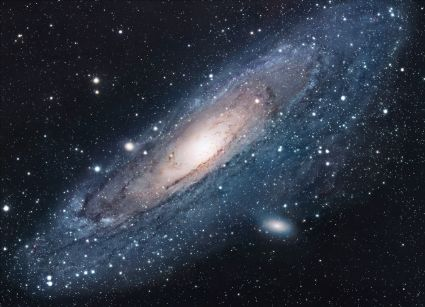
\includegraphics[scale=1.7]{universe}
%\caption{The Universe}
%\label{fig:universe}
%\end{figure}



\bibliographystyle{plain}
\bibliography{alexis,stat}
\end{document}
